The search for six strategies has two motivations. The first is that, as was shown in Section \ref{subsubsec:ParTIptOne} Figure \ref{fig:convexHullCurseOfDimensionality}, for more than five dimensions most points are in the convex set of points and therefore not inside of the Pareto front, unless the number of points becomes very large. As such, this justifies six as an upper bound.
The lower bound is slightly harder to justify, but an argument can be found in the fact that there are five personality factors.
In Section \ref{subsubsec:dimensionsOfPersonality} the Big Five model was presented and it was explained that the covariance of personality descriptive adjectives applied to subjects within a large enough population across a multitude of studies leads to five significant factors of personality.
The ParTI principle states that objectives (here: strategies) are the $d+1$ vertices of the simplex on which points fall in the $d$-dimensional subspace of greatest variance, and since personality varies strongly along five factors, there should not be less than six fundamental personality strategies.

\textbf{Archetypes are computed for multiple datasets to ensure generality}.
Under the assumption that no questionnaire inventory and sample population can provide enough generality to find the fundamental personality archetypes, the ParTI principle is applied to seven different datasets (see Section \ref{sec:datasets}).
The Sensible DTU BF dataset is left out because the population is deemed to specified to produce general enough archetypes.
For each dataset archetypes are computed as median values over 5000 bootstrapping iterations with sample size 200.
The emerging sets of archetypes (median values) are presented in Figure \ref{fig:medianDistances}. Section \ref{subsec:computingConsensusArchetypes} explains in detail how the archetypes are computed.

\begin{figure}
	\centering
	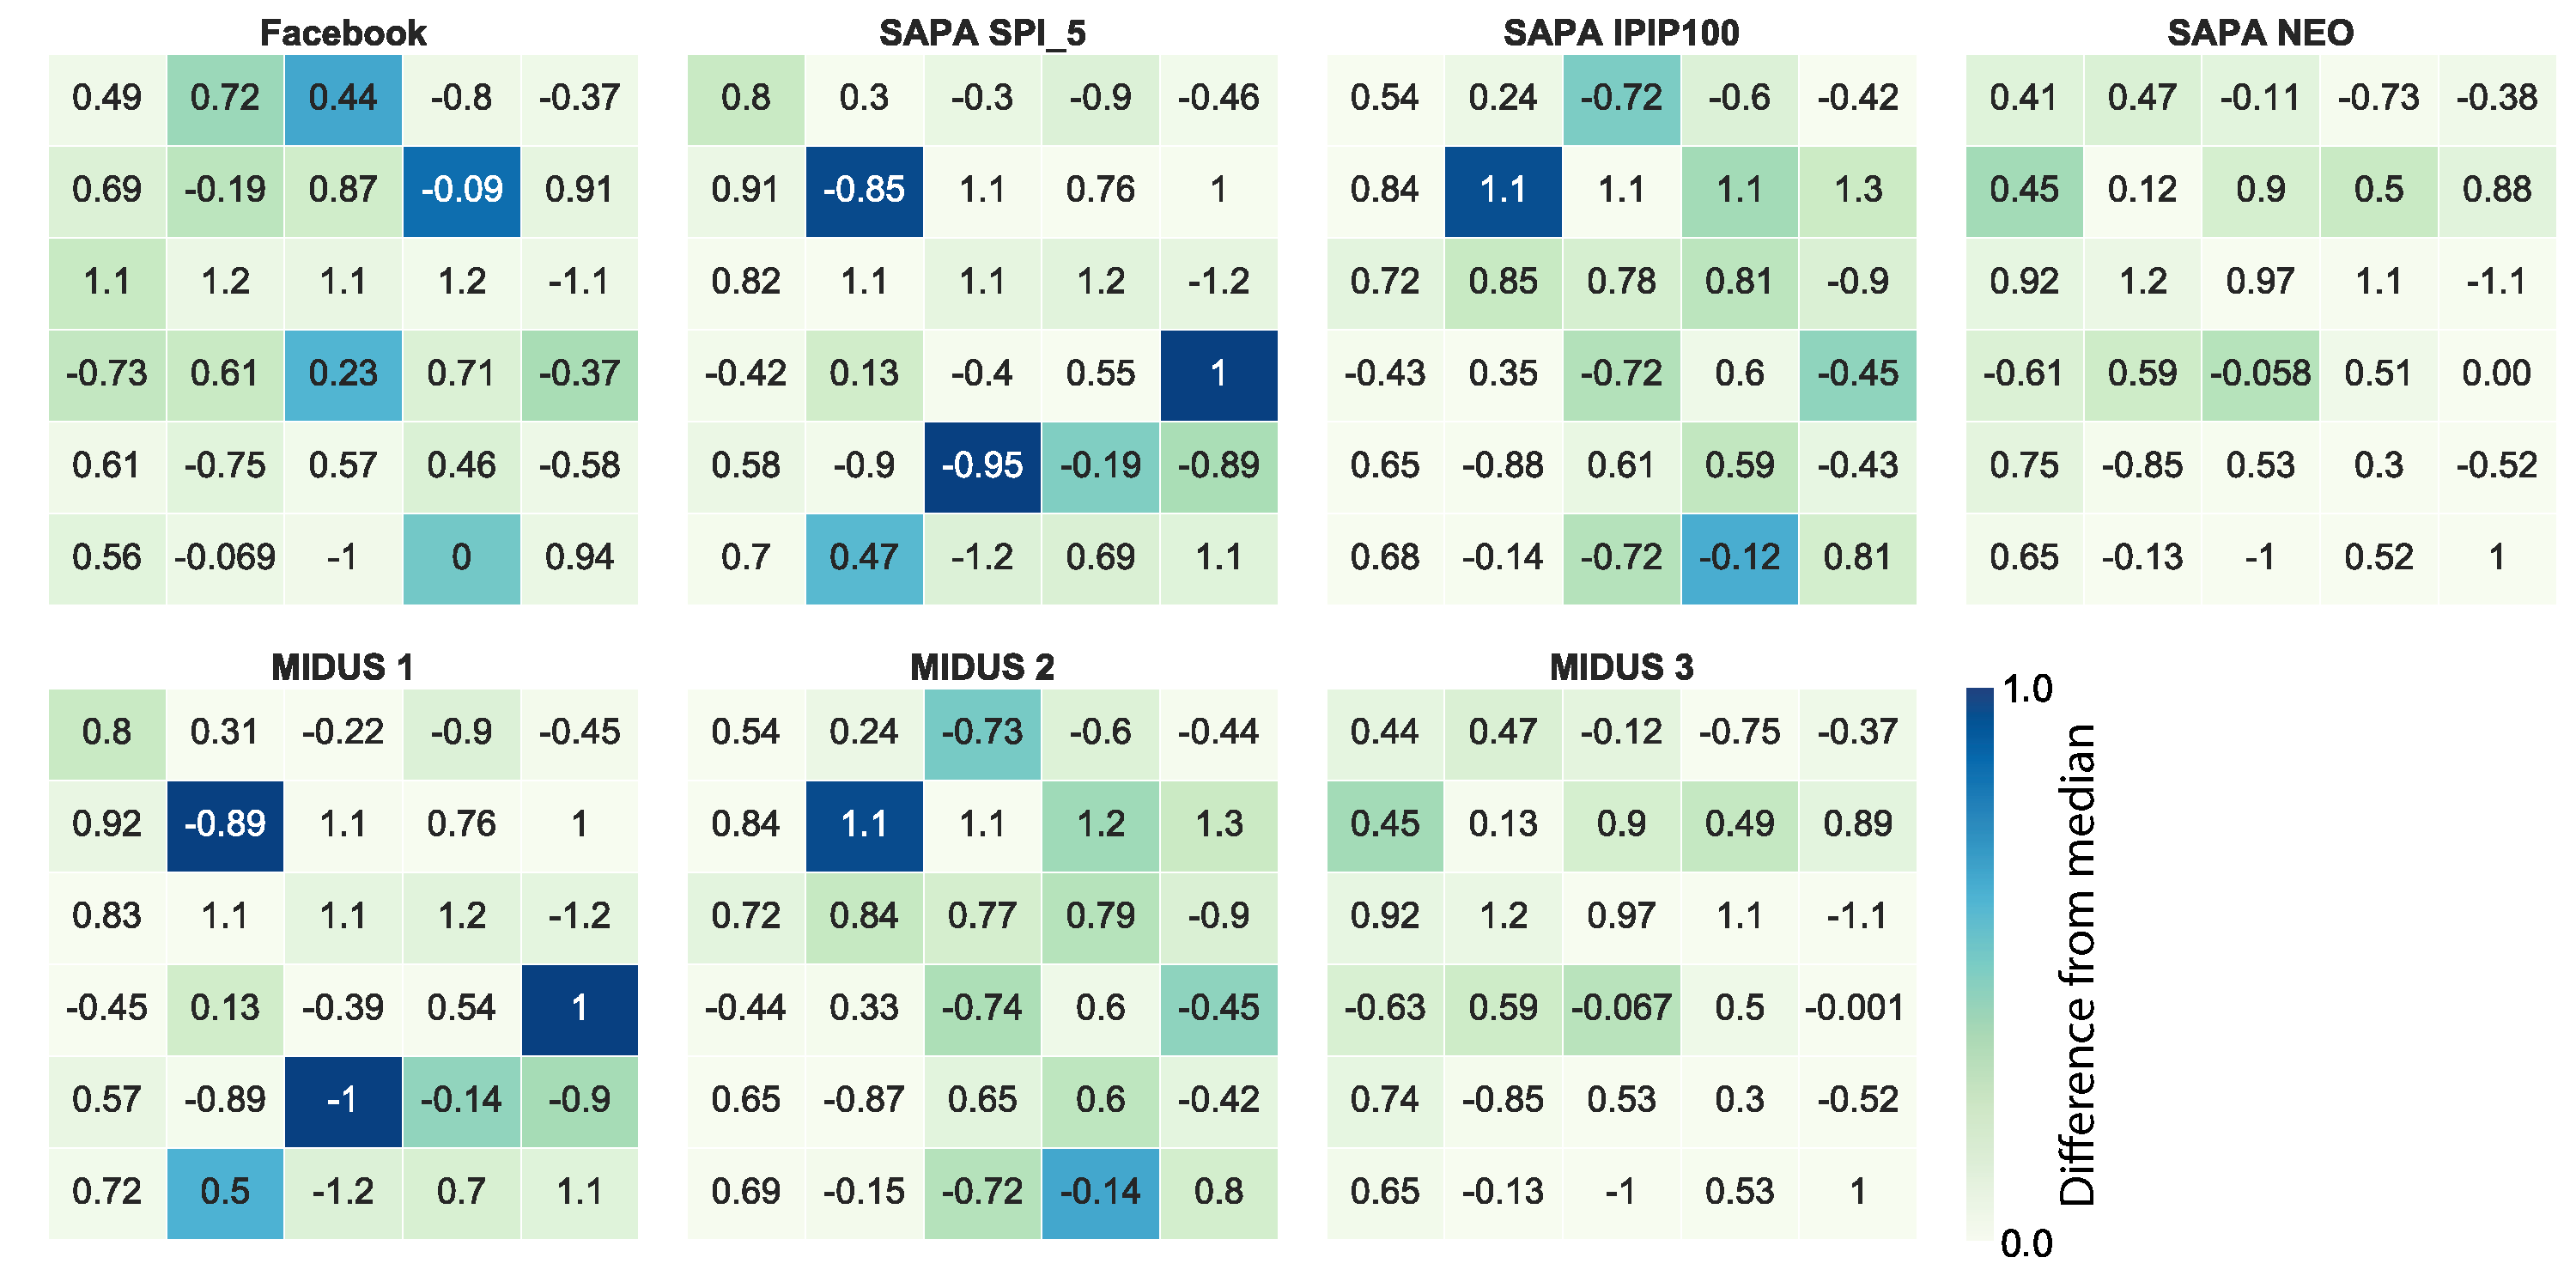
\includegraphics[width=\textwidth]{figures/medianDistances}
	\caption{\label{fig:medianDistances} Archetypes emerging from each dataset.
	Color map scales with archetype trait distances from archetype trait median across all datasets.
	Annotated values are rows of archetypes and BFTs as columns ordered by O, C, E, A and N.}
\end{figure}

\textbf{Archetype deviations across datsets reveal \textit{consensus archetypes}}. 
Figure \ref{fig:medianDistances} shows that roughly the same archetypes emerge from the different datasets.
However, certain archetype traits are far from the median.
Since these are large datasets from mixed populations it is not believed that any one produces archetypes that are severely different due to noise.
Rather the differences are believed more likely to arise due to characteristics relating to the population and the questionnaire inventory.
To investigate the severity of the differences a $6 \times 5$ array of SDs across the datasets (stacked in depth and calculated along 2nd axis, see Section \ref{subsec:computingConsensusArchetypes}) is computed, and shown in Figure \ref{fig:varianceThreshold}.a.
Due to the observation that some archetype traits appear to have much higher SD than others a \textit{consensus threshold} of maximum SD, $\lambda$, is set for a significance level $\alpha = 0.05$.
To find the threshold, an SD value array is computed multiple times for shuffled archetype traits (columns shuffled independently).
All resulting SDs are then arranged in a list and sorted to ascending order, and the largest value of the lower 5th percentile is chosen as the threshold.
This method results in $\lambda = 0.22$.
The distribution of SDs and shuffled archetype SDs are visualized in Figure \ref{fig:varianceThreshold}.b.
Clearly there is a group of archetype traits with low SD and one with high SD.
$\lambda$ gives rise to a mask that decides which archetype traits are in consensus and which are not.
Applying the mask to the median archetypes across all datasets reveals the \textit{consensus archetypes} (CA) presented in Figure \ref{fig:consensusArchetypes}.a.
For consistency the CAs are here named according to their later speculated strategies.\\

\begin{figure}
	\centering
	\begin{minipage}[l]{0.45\textwidth}
		\centering
		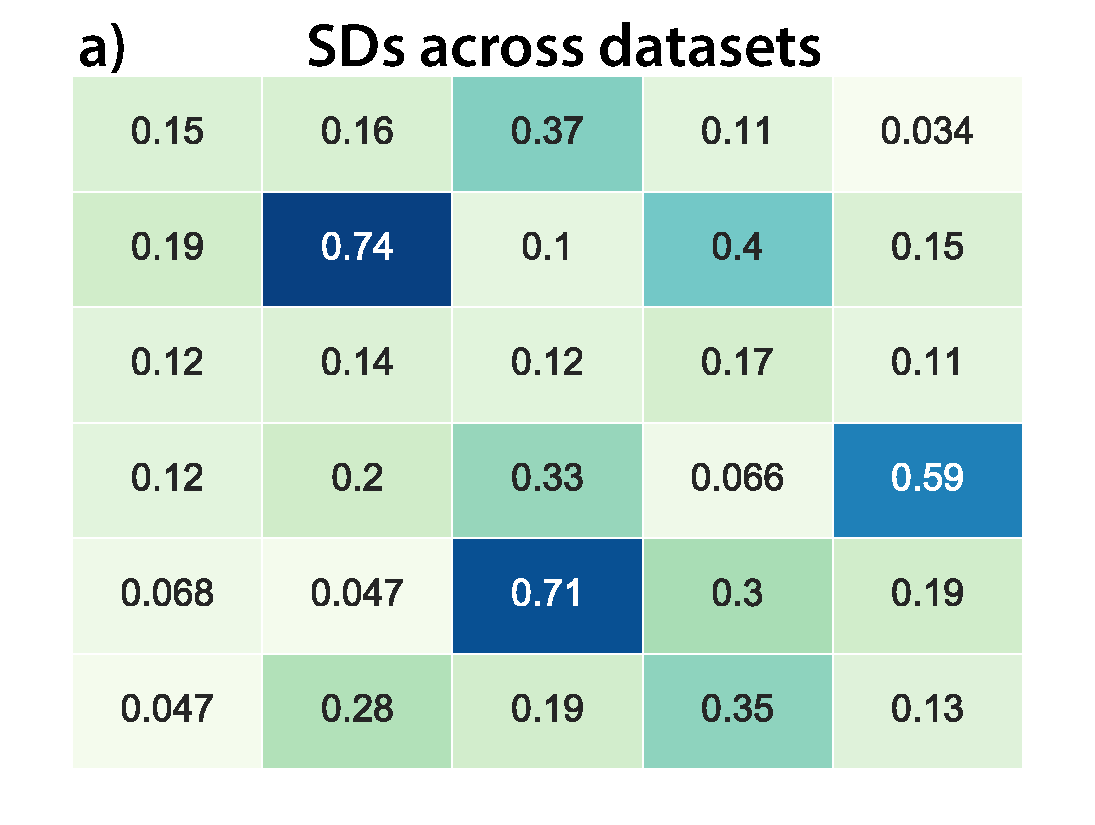
\includegraphics[width=\textwidth]{figures/stdsAcrossDatasets}
	\end{minipage}
	\begin{minipage}[r]{0.52\textwidth}
		\centering
		\vspace{0.2cm}
		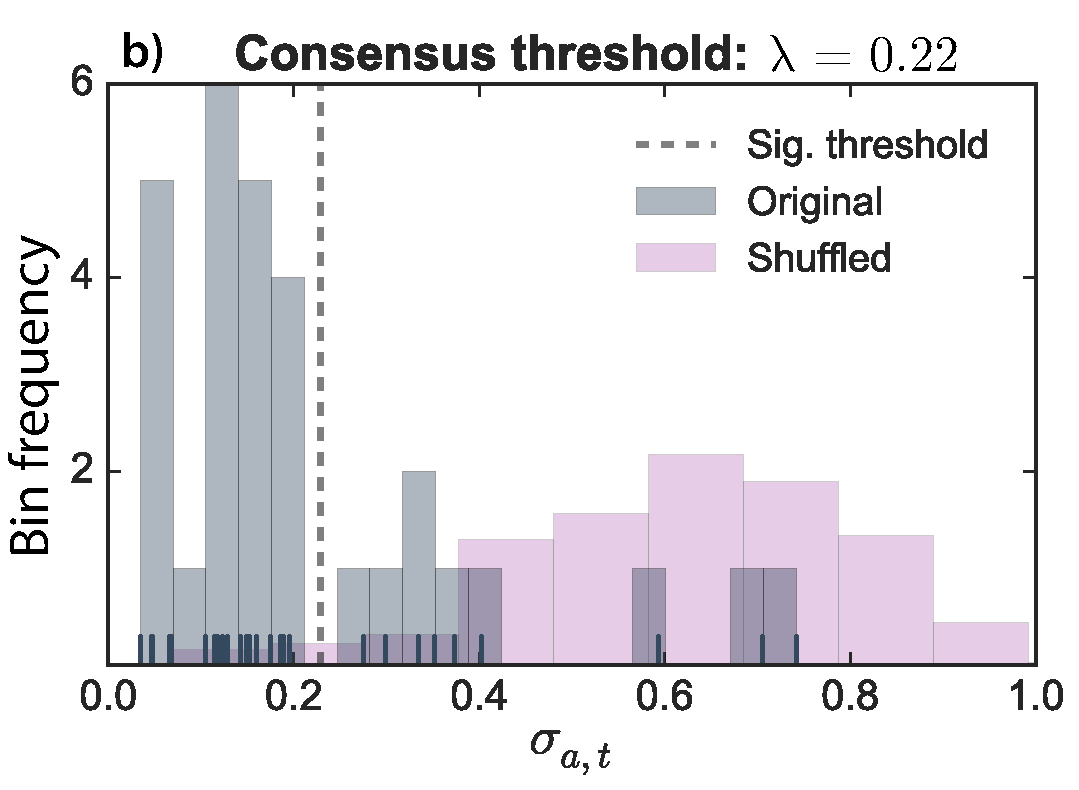
\includegraphics[width=\textwidth]{figures/varianceThreshold}
	\end{minipage}
	\vspace{-0.25cm}
	\caption{\label{fig:varianceThreshold} \textbf{a)} SD values for archetype traits across datasets.
	It is observed that some vary greatly while others are very stable. \textbf{b)} A consensus threshold $\lambda$ emerges at 0.22, which gives rise to $p$-values less than 0.05 for all archetype traits below the consensus threshold.
	The purple histogram shows the normalized distribution of SDs for shuffled archetype traits.
	The blue histogram shows the normalized distribution of SDs of the actual archetypes, where the rug shows distribution of individual SDs.}
\end{figure}

\begin{figure}
	\centering
	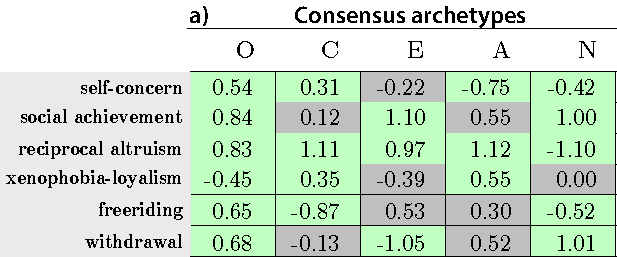
\includegraphics[width=0.7\textwidth]{figures/consensusArchetypes}
	\hspace{0.2cm}
	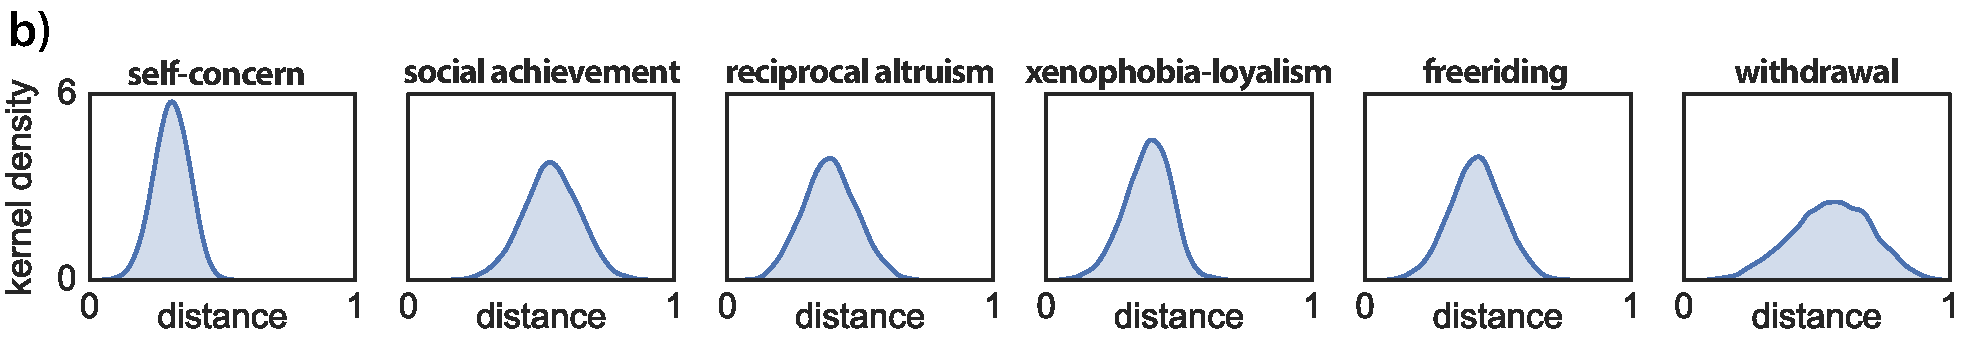
\includegraphics[width=\textwidth]{figures/archetypeDistanceDistributions}
	\caption{\label{fig:consensusArchetypes} \textbf{a)} \textbf{Main result of Section \ref{subsec:consensusArchetypes}}.
	Consensus archetypes emerge as median archetypes where trait values are colored with respect to the consensus threshold: green signifies consensus and gray signifies above threshold non-consensus, i.e.
	undefined dimensions. \textbf{b)} Distributions of weighted euclidean distances from points in the Facebook dataset to consensus archetypes. Axes are scaled equally.}
\end{figure}

The strategies reveal themselves somewhat from the CA traits.
The \achiever CA is particularly unagreeable, which typically correlates with distrust for others and self-centered motives.
The \follower CA is highly introverted and neurotic which could indicate a \textit{constantly-aware-of-danger} strategy.
In fact, it seems, each archetype is quite distinct from the others.
It is definitely worth taking a short break from reading to get acquainted with the CAs and their individual differences and similarities (see Figure \ref{fig:consensusArchetypes}.a).

A remark on the mathematical implications of CAs should be made.
While there are no strict mathematical definitions of what an archetype is, the discourse so far has implied that it is a \textit{point}.
However, once a consensus mask is applied, certain of the trait values for some of the archetypes are said to be "not in consensus".
What this really means is that when e.g. computing the distance to a CA the weighted euclidean distance must be used, adding zero weight to non-consensus traits while all other weights sum to 1.
As such, if, for an archetype, a single trait is in non-consensus the archetype is effectively a line.
If two traits are in non-consensus it is a plane, if three a volume, if four a hyperplane in five dimensions, etc.
In the following analysis the fact that they are CAs and not just normal archetypes only has importance in terms of computing the distance to them, which is done using the weighted euclidean approach as described.
Therefore CAs will be referred to as \textit{archetypes} unless discussion requires them to be explicitly stated as archetypes in consensus between datasets.